% \begin{wrapfigure}[8]{R}{0.4\textwidth}
    % \vspace{-7em}
    % \centering
    % 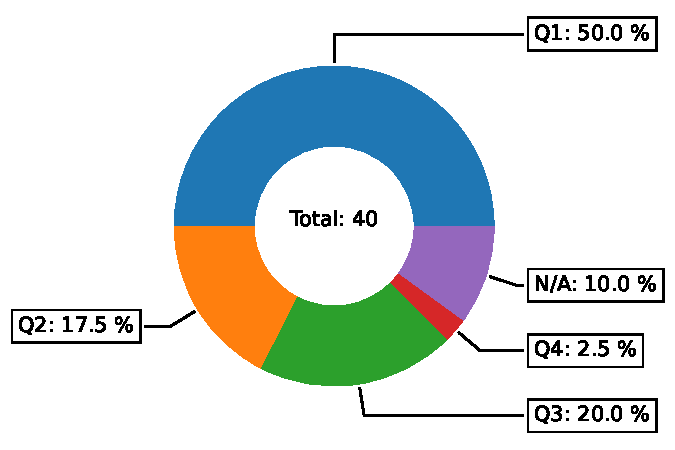
\includegraphics[width=0.98\linewidth]{publicaciones_q.pdf}
    % \caption*{\tiny Ranking de publicaciones con referato según Scimago: \url{https://www.scimagojr.com}.}
% \end{wrapfigure}

\section{Publicaciones científicas y técnicas}

\subsection{Tesis}
 \years{2002} \textbf{Modelo Microscópico de Agua Líquida. Aproximación Esférica Media Generalizada.}
 
 Tesis Doctoral. Facultad de Ciencias Exactas, Universidad Nacional de La Plata. Director: Dr. Fernando Vericat. 

% \fullcite{tesisDoc}
 
 \years{1995} \textbf{Percolación Continua en Fluidos Dipolares.}
 
 Tesis de Grado. Facultad de Ciencias Exactas, Ingeniería y Agrimensura, Universidad Nacional de Rosario. Director: Dr. Fernando Vericat.
 %\fullcite{tesisLic}


\subsection{Artículos publicados en revistas con referato}

% Cuartilos según ranking Scimago\footnote{\url{https://www.scimagojr.com}.}: % $50.0$\% Q1, $17.5$\% Q2, $20.0$\% Q3, $2.5$\% Q4, $10.0$\% N/A.
% \begin{center}
% \begin{tabular}{rlrlrl}
    % Q1: & $50.0$\% & Q3: & $20.0$\% & N/A: & $10.0$\% \\
    % Q2: & $17.5$\% & Q4: & $2.5$\% & \\
% \end{tabular}
% \end{center}

\begin{etaremune}
\item \marginnote{\small{2024}} \fullcite{carlevaro2024}.
\item \marginnote{\small{2023}} \fullcite{basak2023}.
    \item \fullcite{cervantes2023}.
\item \fullcite{alvarez2023}.
\item \fullcite{barbosa2023}.
\item \fullcite{luque2023}.
\item\marginnote{\small{2022}} \fullcite{espinosa2022}.
\item \fullcite{pugnaloni2022}.
\item \fullcite{carlevaro2022}.
\item\marginnote{\small{2021}}\fullcite{basak2021}.
\item \fullcite{espinosa2021}. 
\item \fullcite{madrid2021}.
\item \fullcite{vega2021}.
\item\marginnote{\small{2020}} \fullcite{fajardo2020}
\item \fullcite{carlevaro2020}. 
\item\marginnote{\small{2019}} \fullcite{fajardo2019b}.
\item \fullcite{kozlowski2019}.
\item \fullcite{fajardo2019}.
\item \fullcite{sanchez2019}.
\item \marginnote{\small{2018}}\fullcite{vericat2018}.
\item \fullcite{goldberg2018}.
\item \fullcite{fajardo2018b}.
\item \fullcite{baldini2018}.
\item \fullcite{fajardo2018}.
\item\marginnote{\small{2016}}\fullcite{carlevaro2016b}.
\item \fullcite{kondic2016}.
\item \fullcite{pugnaloni2016}.
\item \fullcite{carlevaro2016}.
\item \marginnote{\small{2015}}\fullcite{goldberg2015}.
\item \marginnote{\small{2014}}\fullcite{irastorza2014}.
\item \marginnote{\small{2013}}\fullcite{irastorza2013b}.
\item \fullcite{sanchez2013b}.
\item \fullcite{irastorza2013}.
\item \fullcite{sanchez2013}.
\item \marginnote{\small{2012}}\fullcite{carlevaro2012b}.
\item \fullcite{carlevaro2012}.
\item \marginnote{\small{2011}}\fullcite{vericat2011}.
\item \fullcite{carlevaro2011}.
\item \marginnote{\small{2010}}\fullcite{stoico2010}.
\item \marginnote{\small{2008}}\fullcite{pugnaloni2008b}.
\item \fullcite{pugnaloni2008}.
\item \fullcite{carlevaro2008}.
\item \marginnote{\small{2004}}\fullcite{carlevaro2004}.
\item \marginnote{\small{2003}}\fullcite{carlevaro2003}.
\item \marginnote{\small{2002}}\fullcite{cetrangolo2002}.
\item \marginnote{\small{2001}}\fullcite{renzi2001}.
\item \marginnote{\small{1998}}\fullcite{carlevaro1998}.
\item \marginnote{\small{1996}}\fullcite{carlevaro1996}.
\end{etaremune}


\subsection{Capítulo de libro}
\textbf{Limitations for Efficiency within the Beef Agrifood Chain in Argentina.}
 
\years{2002} H. Cetrángolo, M. Carlevaro y S. Fernández. En J.H Trienekens y S.W.F. Omta, editores,  \textit{Paradoxes in Food Chains and Networks}, Wageningen Academic Publishers, The Netherlands, pg. 829-839.
 
 \subsection{Informes técnicos}
 \begin{etaremune}
 \item \marginnote{\small{2022}} \fullcite{ytec2022}.
 \item \marginnote{\small{2021}} \fullcite{ytec2021}.
  \item \marginnote{\small{2018}} \fullcite{ytec2018}.
  \item \marginnote{\small{2016}} \fullcite{ytec2016}.
  \item \marginnote{\small{2015}} \fullcite{ytec2015}. 
 \end{etaremune}

 
